\section{Overview}%
\label{sec:chap2Overview}%
\autoBookmark{sec}{Overview}%
This chapter reviews the literature on event classification in Distributed Acoustic Sensing (DAS) in two strands. The first (\refs{sec:chap2ML}) covers the machine-learning foundations of the thesis: the relationship between artificial intelligence, machine learning, and deep learning, and the feature-extraction, feature-selection, class-balancing, and classification components of a signal-classification pipeline. The second (\refs{sec:chap2DAS}) covers the DAS domain: the sensing principle, the signal-processing front end, the transition from classical to deep and graph-based recognition, the constraints of real-time deployment, and the evaluation protocols underlying published results, including the leakage controls on which this thesis builds and the software-engineering perspective on evaluation that it adopts. \refs{sec:chap2RelatedWorks} then tabulates the most relevant studies together with the evaluation protocol of each, \refs{sec:chap2ResearchGap} identifies the three research gaps addressed by RQ1 to RQ3, and \refs{sec:chap2Summary} summarises the chapter.

\section{Machine Learning (ML)}
\label{sec:chap2ML}
\autoBookmark{sec}{ML}
The review of machine learning begins with the relationship between AI, ML, and DL and then considers the components of a signal-classification pipeline in the order in which they operate on a signal. The emphasis throughout is on the methods that the artefact of Chapter~\ref{chap:methodology} instantiates, so that each design decision taken in that chapter can be traced to the literature reviewed here.

\subsection{Artificial Intelligence, Machine Learning, and Deep Learning}
\label{sec:chap2AIMLDL}
\autoBookmark{subsec}{AI, ML, and Deep Learning}
Artificial intelligence is the broad field concerned with systems that perform tasks normally requiring human intelligence. Machine learning is its data-driven subfield, in which predictive mappings are learned from examples rather than programmed as rules. Two ML paradigms are relevant to this thesis. In the classical, feature-based paradigm a domain expert designs descriptors and a comparatively shallow model, such as a support vector machine, random forest, or gradient-boosting ensemble, learns to separate the classes~\cite{breiman2001randomforests,cai2018feature}. In deep learning, multilayer networks learn hierarchical representations directly from raw or lightly processed signals, which reduces manual feature design at the cost of larger models and greater data and computational demands.

Both paradigms have been studied extensively in optical-fibre and acoustic sensing, and recent reviews document a clear migration from handcrafted pipelines towards end-to-end deep models~\cite{venketeswaran2022recent,cao2025aireview}. Convolutional neural networks (CNNs) have become the default choice for spectrogram-based recognition, and recurrent, transformer, and graph architectures are increasingly used to model temporal and spatial dependencies. The two paradigms differ in operational profile: feature-based models tend to be smaller, faster to train, and more interpretable, whereas deep models tend to reach higher peak accuracy but demand more computation and offer less transparency~\cite{shi2025benchmarking}. This trade-off is central to the present work.

The difference in transparency is commonly described as a distinction between white-box and black-box models. A white-box model exposes the basis of its decisions in terms that a person can inspect: a linear model through its coefficients, a decision tree through its split rules, and a feature-based ensemble through the named inputs on which its splits are made. A black-box model, typically a deep network with thousands to millions of weights acting on raw input, learns intermediate representations that have no assigned meaning, so that its decisions can be explained only retrospectively and only approximately~\cite{guidotti2018survey}. Rudin~\cite{rudin2019stop} argues that for high-stakes decisions an interpretable model should be preferred to a black box explained post hoc, because the explanation of a black box need not be faithful to the computation that the model performs. For tree ensembles, Shapley-value attributions can be computed exactly rather than approximated~\cite{lundberg2020trees}, which places gradient-boosted trees over named descriptors considerably closer to the white-box end of this spectrum than a deep network operating on raw signals.

\subsection{Feature Extraction for Signal Classification}
\label{sec:chap2FeatureExtraction}
\autoBookmark{subsec}{Feature Extraction}
Feature extraction transforms a raw signal window into a compact representation suitable for classification. For acoustic and vibration signals, descriptors are conventionally grouped by the domain in which they are computed, and a substantial body of work shows that descriptors from different domains carry complementary information~\cite{sharma2020audio}. The choice of domains therefore determines which aspects of an event a classifier can observe, and a representation that omits a domain cannot recover the information that domain carries.

Time-domain and statistical features (mean, variance, skewness, kurtosis, root-mean-square energy, crest factor, zero-crossing rate, envelope statistics) remain widely used because they are inexpensive to compute and straightforward to interpret~\cite{sharma2020audio,shen2024abnormal}. Frequency-domain descriptors derived from the Fourier transform or power spectral density summarise how vibration energy is distributed across frequencies and separate events with distinct spectral signatures, such as quasi-periodic machinery and impulsive disturbances. Because many real disturbances are non-stationary, time--frequency representations are used to model temporal evolution and spectral content jointly: the short-time Fourier transform (STFT) provides localised spectral views, and wavelet methods (continuous, discrete, and packet transforms) provide a multiresolution characterisation of transient and broadband events~\cite{kandamali2022ml,kozmin2025wavelet}. Cepstral descriptors, notably mel-frequency cepstral coefficients (MFCCs), encode spectral shape compactly and have been transferred from speech to vibration and DAS diagnostics~\cite{han2024intrusion}.

Beyond single-channel descriptors, the distributed nature of DAS supports spatial and spatio-temporal features that treat the measurement as a time--space tensor. Inter-channel coherence, spatial gradients, energy-localisation statistics, and propagation-pattern descriptors improve robustness to noise and fading and help separate localised events from spatially extended activity~\cite{shen2024abnormal,kozmin2025wavelet}. The trend in the literature is therefore away from any single representation and towards multi-domain feature sets.

\subsection{Feature Selection and Dimensionality Reduction}
\label{sec:chap2FeatureSelection}
\autoBookmark{subsec}{Feature Selection}
Large engineered feature sets are frequently redundant and costly, and unselected high-dimensional vectors risk overfitting, particularly in small or imbalanced regimes. Feature selection identifies a compact subset that preserves discriminative power while discarding redundant or irrelevant descriptors~\cite{guyon2003variable,wani2025dimensionality}. Four families are conventionally distinguished. Filter methods score features independently of any classifier. Variance thresholding and Pearson correlation remove near-constant or collinear descriptors; information-theoretic and distance-based filters capture more complex relationships. Mutual information and the minimum-redundancy maximum-relevance (mRMR) criterion select compact subsets that are jointly informative about the label, and ReliefF emphasises features that separate similar instances of different classes~\cite{peng2005mrmr,li2022relieff,altheneyan2025feature}. Wrapper methods such as recursive feature elimination (RFE)~\cite{guyon2002rfe} and Boruta~\cite{kursa2010boruta} evaluate subsets with a specific learner and so account for interactions at greater cost. Embedded methods fold selection into training, and explainability-based approaches, most prominently SHapley Additive exPlanations (SHAP)~\cite{lundberg2017shap}, rank features by their attributed contribution to a trained model's predictions~\cite{cai2018feature}.

Because each criterion embodies different assumptions, no single method is universally optimal, and comparative studies indicate that filter and wrapper methods may select substantially different subsets from the same data~\cite{altheneyan2025feature}. This observation motivates ensemble or consensus selection, in which complementary selectors are combined so that only features supported across multiple paradigms are retained; this is the strategy adopted in the present study. A consensus subset has the further advantage that the retention of each feature can be traced to several independent criteria, which supports the interpretation of the selected descriptors.

\subsection{Class Imbalance Handling}
\label{sec:chap2ClassImbalance}
\autoBookmark{subsec}{Class Imbalance Handling}
Real DAS datasets are typically dominated by background or routine activity, leaving operationally critical events under-represented. If unaddressed, this imbalance biases supervised learning towards the majority class and reduces minority-class recall~\cite{shen2024abnormal}. Two broad classes of remedy are common. Cost-sensitive learning leaves the data unchanged but increases the penalty for minority-class errors, for example through inverse-frequency class weighting. Resampling directly modifies the training distribution: random undersampling discards majority-class samples, whereas oversampling methods such as the Synthetic Minority Over-sampling Technique (SMOTE)~\cite{chawla2002smote} and its variants, Borderline-SMOTE~\cite{han2005borderline} and SMOTE-Tomek~\cite{batista2004balancing}, synthesise minority-class samples by interpolation. These variants may restrict synthesis to decision-boundary regions or remove ambiguous sample pairs. Each strategy balances minority-class sensitivity against the risk of synthetic artefacts and additional training cost; the optimal choice is therefore dataset-dependent, which justifies the empirical comparison undertaken in this study.

\subsection{Classification Algorithms}
\label{sec:chap2Classifiers}
\autoBookmark{subsec}{Classification Algorithms}
A wide range of classifiers has been applied to acoustic and vibration recognition. Logistic regression and single decision trees are fast and interpretable but limited in their capacity to model non-linear interactions. Ensemble methods address this limitation: bagging methods such as random forests and extremely randomised trees reduce variance~\cite{breiman2001randomforests,geurts2006extremely}, and gradient-boosting machines~\cite{friedman2001greedy}, including XGBoost~\cite{chen2016xgboost}, histogram-based gradient boosting, and LightGBM~\cite{ke2017lightgbm}, build additive models that consistently rank among the strongest on tabular feature sets. Such ensembles are well suited to deployment because they combine competitive accuracy with low inference cost and native feature-importance estimates.

In deep learning, CNNs dominate spectrogram- and waveform-based DAS recognition, and hybrid CNN--recurrent, transformer, state-space, and graph architectures have been explored to capture longer-range and cross-channel structure. Comparative benchmarking becomes more important as the number of candidate models grows: a recent comparison of convolutional, recurrent, transformer, and classical models on DAS data found that no single architecture dominates under all conditions~\cite{shi2025benchmarking}, and low-code AutoML libraries have lowered the barrier to such comparisons~\cite{ali2020pycaret}. Whether observed differences are systematic is usually assessed with the non-parametric procedures of Dem\v{s}ar~\cite{demsar2006statistical}, namely the Friedman test with post-hoc Nemenyi analysis. These procedures assume that the blocks over which classifiers are ranked are independent replicates, an assumption that a single partition of one dataset does not satisfy (\refss{sec:chap2LeakStatistics}); \refss{sec:chap3Statistics} returns to this point.

\section{Distributed Acoustic Sensing (DAS)}
\label{sec:chap2DAS}
\autoBookmark{sec}{DAS}
The review of the DAS domain proceeds from the sensing principle of the fibre, through the classifiers that have been built on its signal, to the manner in which those classifiers have been evaluated. This final topic leads directly to the evaluation gap identified at the end of the chapter.

\subsection{Principles of DAS and \texorpdfstring{$\Phi$-OTDR}{Phi-OTDR}}
\label{sec:chap2DASprinciples}
\autoBookmark{subsec}{Principles of DAS}
DAS converts a standard optical fibre into a continuous array of virtual acoustic sensors. An interrogator launches coherent laser pulses into the fibre and analyses the Rayleigh backscatter produced by refractive-index inhomogeneities along the glass using phase-sensitive optical time-domain reflectometry ($\Phi$-OTDR)~\cite{he2021review,liu2025advances}. Acoustic and seismic disturbances near the fibre strain the glass and modulate the phase of the backscattered light, so that vibrations can be localised and quantified along the entire cable~\cite{hartog2017introduction}. A single interrogator monitors tens of kilometres at metre-scale resolution in real time, which has made DAS a major research frontier~\cite{shang2022das} with applications in pipeline surveillance, railway protection, road-traffic monitoring, and perimeter intrusion detection~\cite{wu2024pipeline,yurekli2025railway,deng2025roadtraffic,juarez2005intrusion}. The sensitivity of the fibre is directional: axial strain is sensed far more strongly than broadside strain, so that a given event produces a weaker signature when it acts perpendicular to the cable~\cite{zhan2020das}.

\begin{figure}[!htbp]
\centering
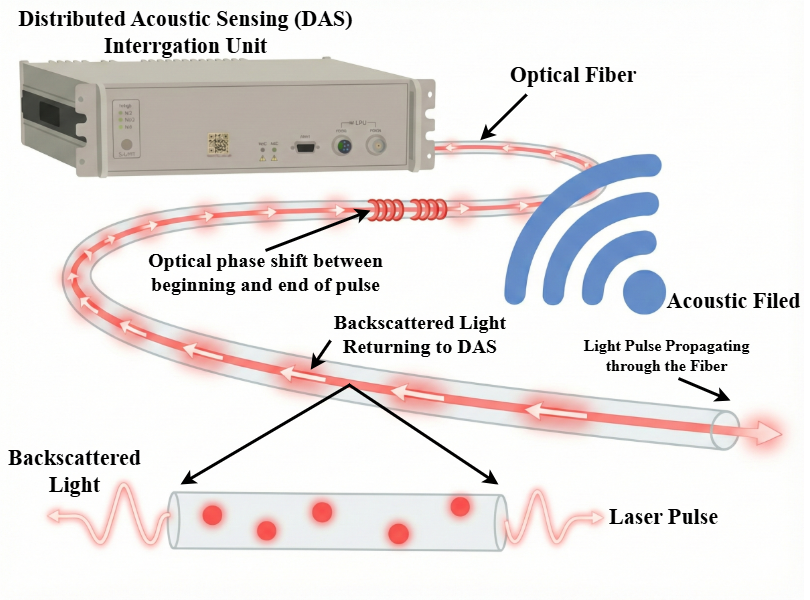
\includegraphics[width=0.85\textwidth]{Figures/fig01_DAS.png}
\caption{Distributed acoustic sensing system.}
\label{fig:das-system}
\end{figure}

For analysis, DAS measurements are commonly represented as spatio-temporal distance--time maps or as time--frequency matrices from which descriptors are derived~\cite{kandamali2022ml}. This representation underpins the multi-domain design adopted in this thesis, in which one window is described simultaneously in the time, frequency, time--frequency, and spatial domains. The breadth of DAS applications has also motivated dedicated reviews of DAS methodologies and deep-learning approaches, including in subsurface settings~\cite{shahabudin2025review}.

\subsection{DAS Signal Processing}
\label{sec:chap2DASsignal}
\autoBookmark{subsec}{DAS Signal Processing}
Raw $\Phi$-OTDR signals are high-dimensional and noisy, and front-end processing therefore aims to raise the signal-to-noise ratio, mitigate coherent fading, and convert backscatter into representations suitable for classification~\cite{kandamali2022ml}. Typical pipelines apply temporal and spatial band-pass filtering, amplitude normalisation, and channel selection or aggregation. To address the non-stationarity of footsteps, vehicles, and excavation, STFT- or wavelet-based time--frequency analysis is widely used. The choice and ordering of these operations are consequential, because any component of the raw measurement that survives preprocessing is absorbed into the descriptors as though it were information about the event.

Early long-perimeter intrusion systems combined handcrafted features such as energy, spectral amplitude, and variance with fixed thresholds and spatial-consistency checks; these systems performed adequately in controlled settings but degraded under environmental variability, which motivated adaptive, learning-based methods~\cite{juarez2005intrusion}. Learned denoising has since been proposed, for example with densely connected residual convolutional networks~\cite{huang2024noise}. The preprocessing chain in this thesis follows the same principles, combining DC-offset removal, Butterworth band-pass filtering, and z-score normalisation, with the normalisation step additionally serving as a leakage control (\refss{sec:chap3Normalisation}).

\subsection{Event Classification Using Classical Machine Learning}
\label{sec:chap2DASclassicalML}
\autoBookmark{subsec}{Classical ML for DAS}
A substantial body of work pairs handcrafted features with classical models, following the general workflow illustrated in \reff{fig:das_machine_learning}. Bublin demonstrated that knowledge-based features combined with classical ML and deep learning could exceed $99.9\%$ accuracy on binary excavator detection, using Fourier and RMS descriptors together with image-derived features~\cite{bublin2021event}, and had earlier compared classical, image-based, and deep approaches more broadly~\cite{bublin2019ml}. Cao et al.\ released an open six-class $\Phi$-OTDR dataset with SVM and CNN baselines, the SVM operating on 16 handcrafted statistical and spectral features~\cite{caoxin2023opendataset}. For urban traffic, Min et al.\ extracted vehicle signals by filtering and scaling ahead of a radial-basis-function SVM~\cite{min2024vehicle}. Shen et al.\ reduced time-domain statistics and fed them, together with a convolutional-recurrent encoder, into a gradient-boosting classifier for imbalanced fibre-vibration data~\cite{shen2024abnormal}, and Kozmin et al.\ combined wavelet packet decomposition and PCA with a hybrid logistic-regression and residual-CNN model~\cite{kozmin2025wavelet}. These studies establish that carefully engineered descriptors combined with lightweight classifiers are effective for DAS event discrimination, particularly when the number of classes is small.

\begin{figure}[!htbp]
\centering
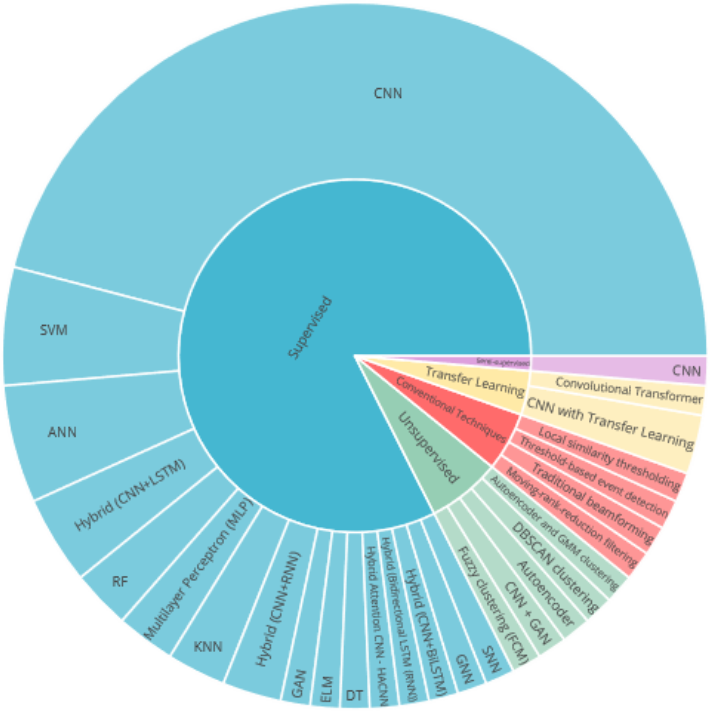
\includegraphics[width=0.68\textwidth]{Figures/fig02_ML_classification.png}
\caption{Machine learning workflow for event detection and classification \cite{shahabudin2025review}.}
\label{fig:das_machine_learning}
\end{figure}

\subsection{Event Classification Using Deep Learning and Graph Models}
\label{sec:chap2DASdeepLearning}
\autoBookmark{subsec}{Deep Learning for DAS}
More recent work applies supervised deep learning directly to DAS spectrograms or distance--time representations~\cite{tomasov2023enhancing,tomasov2025perimeter}. Convolutional long short-term memory networks have been used for temporal modelling in railway intrusion detection~\cite{li2020convlstm}, and deep models have been deployed for intrusion detection and impulsive-event classification across operational telecommunications networks~\cite{han2024intrusion}. Semi-supervised learning has been explored to reduce annotation demands, for example for rock-slope failure monitoring~\cite{kang2024semisupervised}.

Transformer and graph architectures now set the reported state of the art on the public campus benchmark used in this thesis. Dione et al.\ introduced DASViT1D, a one-dimensional vision transformer over multi-domain (MFCC, RDFT, DWT) inputs, reporting $93.5\%$ accuracy on the nine-class taxonomy~\cite{dione2025intrusion}, and later DAStatFormer, a multi-branch transformer that integrates 24 statistical features per channel, reporting $99.93\%$~\cite{dione2026dastatformer}. Jeong et al.\ proposed S2-DyGNN, a spectro-spatial dynamic graph neural network that treats the channel axis as a graph and reports $94.0\%$, alongside graph attention and graph convolutional baselines~\cite{jeong2026s2dygnn}; graph neural networks have also been applied to microseismic event detection in DAS data~\cite{shahabudin2024gnn}. A benchmark comparing convolutional, recurrent, transformer, state-space, and classical models found no single architecture best under all conditions~\cite{shi2025benchmarking}. These figures are not directly comparable with one another, because each is obtained under its own partition, window density, and taxonomy; \refs{sec:chap2RelatedWorks} records the protocol alongside each result for that reason.

\subsection{Real-Time and Deployment Considerations}
\label{sec:chap2DASdeployment}
\autoBookmark{subsec}{Real-Time and Deployment Considerations}
Recognition accuracy is necessary but insufficient for operational monitoring, which imposes constraints on latency, throughput, bandwidth, and energy consumption across sensing, transport, storage, and inference~\cite{deng2025roadtraffic}. Deep networks tailored to DAS can achieve high accuracy but often require hardware accelerators and further optimisation to satisfy deployment constraints; they also remain susceptible to dataset shift and calibration drift~\cite{shi2025benchmarking}. These considerations have motivated both efficient deep architectures and feature-engineered pipelines for which the cost of each processing stage can be quantified explicitly. Production studies of DAS road-traffic systems identify inference-pipeline design and buffered pre-computation as key engineering challenges~\cite{deng2025roadtraffic}, while hybrid ensembles have demonstrated reliable real-time hazard detection on railways~\cite{yurekli2025railway}. Few studies report the online computational cost of the complete pipeline rather than that of the classifier alone; those that provide timing data generally report only inference cost.

Lightness is therefore claimed more often than it is measured. A model may be light in one respect and heavy in another: a network with few parameters may still require many hours of GPU training, and a classifier that predicts within microseconds may depend on an input transform that dominates the processing time per window. A complete account of the footprint of a model requires four quantities: the stored size of the trained model, the per-window inference latency, the end-to-end latency including the preparation of the input, and the training time together with the hardware it requires. Only a comparison of models on all four quantities, on the same hardware, allows a claim of lightness to be verified. This thesis adopts that account (\refs{sec:ResearchBackground}) and applies it to the pipeline and to every baseline.

\subsection{Evaluation Protocols and Data Leakage}
\label{sec:chap2Leakage}
\autoBookmark{subsec}{Evaluation Protocols and Data Leakage}
Data leakage is the unintended transfer of information from evaluation data into model training, so that a model is assessed with information it could not legitimately possess at deployment~\cite{kaufman2012leakage}. It is a recognised cause of overly optimistic and irreproducible results in applied machine learning: a review of machine-learning-based science found leakage in at least 294 published studies across seventeen fields and organised it into a taxonomy whose forms include preprocessing and feature selection fitted on training and test data together, temporal leakage, and non-independence between training and test samples~\cite{kapoor2023leakage}. Three families of leakage are relevant to DAS event classification: leakage through dependent samples, leakage through the modelling pipeline, and leakage into the statistical comparison of methods. The subsections below review the controls that the literature recommends for each family, and Table~\ref{tab:leakage_controls} relates every control to its implementation in Chapter~\ref{chap:methodology}.

\begin{table}[!htbp]
	\centering
	\caption{Leakage pathways relevant to DAS event classification, the controls recommended in the literature, and their implementation in this thesis.}
	\label{tab:leakage_controls}
	\footnotesize
	\setlength{\tabcolsep}{4pt}
	\renewcommand{\arraystretch}{1.15}
	\begin{tabularx}{\textwidth}{@{}>{\raggedright\arraybackslash}p{2.3cm} >{\raggedright\arraybackslash}X >{\raggedright\arraybackslash}X >{\raggedright\arraybackslash}X@{}}
		\toprule
		\textbf{Pathway} & \textbf{Mechanism} & \textbf{Recommended control} & \textbf{Implementation in this thesis}\\
		\midrule
		Overlapping windows & Random window-level splits place near-duplicate windows in training and test & Blocked partitions with a gap between training and test blocks~\cite{burman1994hblock,racine2000hvblock,bergmeir2012timeseries,dehghani2019windows} & Blocked segments with one-window guard bands; raw-sample disjointness asserted (Sec.~\ref{sec:chap3Partitioning})\\
		\addlinespace[3pt]
		Recording or session dependence & Samples from one recording appear in both training and test & Partitioning by subject, session, or recording~\cite{saeb2017usecase,roberts2017crossvalidation} & Session-grouped (Cao) and recording-segment (Tomasov) partitions; leave-one-date-out and leave-one-recording-out evaluation (Secs.~\ref{sec:chap3Partitioning} and~\ref{sec:chap3ConfoundDesign})\\
		\addlinespace[3pt]
		Feature selection outside the training fold & Selection uses rows that are later used for evaluation & Selection repeated inside every training fold~\cite{ambroise2002selection} & Selectors fitted on training rows and refitted per fold (Sec.~\ref{sec:chap3FeatureSelection})\\
		\addlinespace[3pt]
		Model selection on evaluation data & Configurations are chosen on the data used to report performance & Separate validation data or nested cross-validation~\cite{varma2006bias,cawley2010overfitting} & Selection on the validation set; test scores reported once (Sec.~\ref{sec:chap3ModelReady})\\
		\addlinespace[3pt]
		Resampling before partitioning & Synthetic samples interpolate across the split & Resampling inside the training fold only~\cite{santos2018imbalanced} & Resamplers inside the training pipeline (Sec.~\ref{sec:chap3Balancing})\\
		\addlinespace[3pt]
		Preprocessing fitted on all data & Scaling statistics include evaluation rows & Preprocessing fitted on training data alone~\cite{kapoor2023leakage} & Stateless per-window preprocessing; scaler inside the training pipeline (Secs.~\ref{sec:chap3Preprocessing} and~\ref{sec:chap3ModelReady})\\
		\addlinespace[3pt]
		Dependent units in statistics & Tests and intervals treat dependent results as independent & Independent replicates, corrected tests, and cluster resampling~\cite{dietterich1998tests,nadeau2003inference,field2007clustered} & Repeated partitions, group bootstrap, and paired tests over held-out acquisitions (Sec.~\ref{sec:chap3Statistics})\\
		\bottomrule
	\end{tabularx}
\end{table}

\subsubsection{Leakage Through Dependent Samples}
\label{sec:chap2LeakDependent}
\autoBookmark{subsubsec}{Leakage Through Dependent Samples}
The first family arises when training and test samples are not independent. Roberts et al.~\cite{roberts2017crossvalidation} demonstrate that, for temporally, spatially, and hierarchically structured data, random cross-validation systematically overestimates predictive performance, and they recommend blocked partitions whose boundaries follow the dependence structure of the data. For serially dependent observations, h-block cross-validation removes a band of observations on either side of each test observation so that no training observation lies close to it~\cite{burman1994hblock}, hv-block cross-validation extends the idea to consistent model selection~\cite{racine2000hvblock}, and blocked schemes of this kind give more reliable error estimates for time-series predictors than random partitioning~\cite{bergmeir2012timeseries}. When several samples are drawn from one subject, the corresponding requirement is that the split be made by subject rather than by record: in clinical sensor data, record-wise cross-validation substantially overestimates the accuracy that subject-wise cross-validation measures~\cite{saeb2017usecase}. Sliding-window segmentation compounds the problem, because overlapping windows from one stream are near-duplicates, and the apparent benefit of overlapping windows in human activity recognition has been traced to evaluation schemes that do not keep the windows of one subject together~\cite{dehghani2019windows}.

These findings transfer directly to DAS. Overlapping analysis windows are serially dependent observations in the sense of h-block cross-validation, so a gap of at least one window length between training and test windows plays the role of the removed band. A recording session plays the role of the clinical subject, so the session or recording, rather than the window, is the natural unit of partitioning. The partitions of Chapter~\ref{chap:methodology} apply both principles, grouping Cao records by session and dividing each Tomasov recording into blocked segments separated by guard bands.

\subsubsection{Leakage Through the Modelling Pipeline}
\label{sec:chap2LeakPipeline}
\autoBookmark{subsubsec}{Leakage Through the Modelling Pipeline}
The second family arises when a fitted component of the pipeline is exposed to data that are later used for evaluation. Feature selection performed on the full dataset before cross-validation is the best-known case: in microarray classification it severely underestimates the error rate, and an unbiased estimate requires selection to be repeated within every training fold~\cite{ambroise2002selection}. Using cross-validation both to tune a model and to estimate its error introduces a comparable optimistic bias~\cite{varma2006bias}, and selecting among many configurations on the data used to report performance overfits the selection criterion itself~\cite{cawley2010overfitting}. Resampling for class imbalance creates a further pathway, because oversampling before partitioning places synthetic samples derived from evaluation instances in the training data and yields over-optimistic estimates~\cite{santos2018imbalanced}. The common remedy is to treat every data-dependent operation, including scaling, feature selection, and resampling, as part of the model, fitting it on training data alone and applying it unchanged to evaluation data~\cite{kapoor2023leakage}. Chapter~\ref{chap:methodology} adopts this principle throughout and also measures the bias that feature selection outside the cross-validation loop would introduce.

\subsubsection{Leakage into Statistical Comparison}
\label{sec:chap2LeakStatistics}
\autoBookmark{subsubsec}{Leakage into Statistical Comparison}
The third family concerns the statistics used to compare methods, which assume that the units over which they are computed are independent. Dietterich~\cite{dietterich1998tests} showed that several widely used tests for comparing classifiers, including the resampled paired $t$-test, have an elevated Type~I error because their samples share data, and Nadeau and Bengio~\cite{nadeau2003inference} showed that the overlap between training sets in repeated resampling causes the variance of the estimated generalisation error to be underestimated, and proposed a corrected test. For comparing several classifiers across several datasets, Dem\v{s}ar~\cite{demsar2006statistical} recommends the Friedman test with post-hoc Nemenyi analysis, with the datasets serving as independent blocks, together with step-down procedures such as Holm's for families of pairwise comparisons~\cite{holm1979simple}. Where observations are clustered, as windows are within recordings, resampling should operate on whole clusters so that bootstrap intervals reflect the dependence between observations~\cite{field2007clustered}. The statistical procedures of Chapter~\ref{chap:methodology} follow these principles by replicating over independently generated partitions and independent acquisitions rather than over configurations of a single partition.

\subsubsection{Leakage in Published DAS Benchmarks}
\label{sec:chap2LeakDAS}
\autoBookmark{subsubsec}{Leakage in Published DAS Benchmarks}
In DAS, the dependence structure that makes these controls necessary is physical rather than incidental. Overlapping analysis windows share raw interrogator samples, and all samples from a given recording session share the fibre state, coupling, interrogator configuration, and ambient conditions~\cite{tomasov2025dataset,caoxin2023opendataset}. Distributing such dependent samples across partitions enables a model to exploit recording-specific structure rather than event characteristics. The public datasets used in this thesis illustrate both mechanisms. Cao et al.~\cite{caoxin2023opendataset} release a fixed $8{:}2$ partition of $15{,}419$ pre-segmented records and report SVM and CNN baselines on it. Tomasov et al.~\cite{tomasov2025perimeter} generate classification vectors by sliding an $8{,}192$-sample window with a 256-sample stride, a $96.9\%$ overlap, and evaluate with random 10-fold cross-validation. Neither protocol constrains samples from one continuous recording to one side of the partition. Later studies adopt partial controls: Dione et al.~\cite{dione2025intrusion} fit their scaler on training folds only but do not address window or recording overlap, and Jeong et al.~\cite{jeong2026s2dygnn} use a chronological split with a five-window guard band, which removes window overlap at the boundary but still places segments of every recording on both sides. No study in Table~\ref{tab:relatedworks} groups its partition by recording, session, or acquisition date, and none reports verifying that its test set is disjoint from its training set at the level of raw measurements.

Reporting practice compounds the problem. A study that evaluates only within the campaign that produced its training data characterises performance at a site already represented in training, not at a new site. Both quantities are useful, but they answer different questions and, as Chapter~\ref{chap:ResultsAndDiscussion} shows, differ substantially in magnitude. This gap is methodological rather than algorithmic. It cannot be closed by improved features or larger models; it requires partitioning that respects the dependence structure, verification that the partition achieves what it claims, and reporting that states which protocol produced which result.

\subsubsection{Evaluation as a Software Engineering Concern}
\label{sec:chap2LeakSoftware}
\autoBookmark{subsubsec}{Evaluation as a Software Engineering Concern}
Software-engineering research on machine-learning systems offers a means of making such verification routine. Sculley et al.~\cite{sculley2015debt} describe how data dependencies and pipeline complexity accumulate as hidden technical debt that conventional code review does not reveal, and Breck et al.~\cite{breck2017mltest} respond with a rubric of concrete tests for the data, model, and infrastructure of a production system. The NeurIPS reproducibility programme applies a similar principle to research by requiring that published claims be accompanied by code and a checklist~\cite{pineau2021reproducibility}. The common principle is that a property of a machine-learning system should be tested rather than asserted. This principle has not yet been adopted in DAS event classification, where the validity of an evaluation is stated in a sentence of prose, if it is stated at all. This thesis adopts it directly by implementing its leakage controls as assertions within the pipeline (\refss{sec:chap3Partitioning}), which converts a protocol description into a property that a reader can verify.

\section{Summary of Related Works}
\label{sec:chap2RelatedWorks}
\autoBookmark{sec}{Summary of Related Works}
Table~\ref{tab:relatedworks} consolidates the most relevant prior studies, recording for each the event taxonomy, feature representation, model, reported accuracy, evaluation protocol, and whether leakage was controlled. Because the protocols, datasets, and taxonomies differ, the reported accuracies provide context rather than a ranking, and this thesis draws no comparison between them. Two observations emerge. High accuracies are most often reported for tasks with few, well-separated classes, and the strongest recent results on the nine-class campus benchmark are obtained by high-capacity transformer and graph models evaluated under random or chronological partitions of overlapping windows.

\begin{landscape}
\begin{table}[p]
\centering
\caption{Summary of related works on DAS event classification, with the evaluation protocol of each study.}
\label{tab:relatedworks}
\scriptsize
\setlength{\tabcolsep}{4pt}
\renewcommand{\arraystretch}{1.2}
\begin{tabular}{@{}>{\raggedright\arraybackslash}p{2.3cm} >{\raggedright\arraybackslash}p{2.8cm} >{\raggedright\arraybackslash}p{3.7cm} >{\raggedright\arraybackslash}p{4.2cm} >{\raggedright\arraybackslash}p{3.4cm} >{\raggedright\arraybackslash}p{3.7cm}@{}}
\toprule
\textbf{Study (Year)} & \textbf{Dataset (labels)} & \textbf{Feature representation} & \textbf{Model and reported accuracy} & \textbf{Evaluation protocol} & \textbf{Leakage control}\\
\midrule
Bublin (2021)~\cite{bublin2021event} & Own; 2 (excavator vs.\ none) & FFT; RMS windows; Sobel image features & kNN 99.96\%, RF 99.95\%, CNN 99.91\% & Random split & Not reported\\
Cao et al.\ (2023)~\cite{caoxin2023opendataset} & Cao; 6 & 16 handcrafted statistical/spectral (1D); raw time--space matrices (2D) & SVM, CNN & Random 8:2 over pre-segmented records & No; 423 of 441 sessions contribute to both folders\\
Tomasov et al.\ (2023)~\cite{tomasov2023enhancing} & Tomasov; 7 & Hann window; oversampled DFT; band-limited power (50--500\,Hz) & CNN, 91.4\% & Random 8:2 over pre-segmented records & No\\
Han et al.\ (2024)~\cite{han2024intrusion} & Own; 2 (intrusion, impulsive events) & HPF, STFT, mel spectrogram, MFCC & ConvNets, ViT, RF; 95\% & Random split & Not reported\\
Min et al.\ (2024)~\cite{min2024vehicle} & Own; 2 (vehicle vs.\ noise) & Low-pass, FK/FX/dip filters, scaling & SVM (RBF); 80\% & Random split & Not reported\\
Shen et al.\ (2024)~\cite{shen2024abnormal} & Own; 2 (human vs.\ natural) & 16-D time statistics reduced to 6-D & ConvLSTM encoder + XGBoost; 99.1\% & Random split & Not reported\\
Kozmin et al.\ (2025)~\cite{kozmin2025wavelet} & Own; 3 (digging, footsteps, noise) & WPD features; PCA & Logistic regression + ResNet CNN; 98\% & Random split & Not reported\\
Shi \& Zong (2025)~\cite{shi2025benchmarking} & Own; 4 & CSDM phase maps; VAE compression & ResNet 95.8\%, MLP 95.3\%, others & Random split & Not reported\\
Tomasov et al.\ (2025)~\cite{tomasov2025perimeter} & Tomasov; 9 & FFT, RDFT, DWT, MFCC & 1D CNN, XGBoost; MFCC 85.61\%, RDFT 85.47\% & Random 10-fold CV, 80/10/10, 8{,}192-sample windows at 256-sample stride (96.9\% overlap) & No; 100\% of test windows share raw samples with training (\refs{sec:resLeakage})\\
Dione et al.\ (2025)~\cite{dione2025intrusion} & Tomasov; 9. Cao; 6 & Multi-domain fusion (MFCC, RDFT, DWT) & DASViT1D; 93.5\% & Fixed 80/10/10 into ``non-overlapping subsets'' & Partial; scaler fitted on training folds only, window and recording overlap not addressed\\
Jeong et al.\ (2026)~\cite{jeong2026s2dygnn} & Tomasov; 9. Cao; 6 & STFT spectrograms; 2D frequency--time CNN features & S2-DyGNN; 94.0\% (GAT 81.2\%, GCN 85.3\%) & Chronological 80/10/10 with a 5-window guard band & Windows yes, recordings no; split is chronological within the stream, not grouped by recording\\
Dione et al.\ (2026)~\cite{dione2026dastatformer} & Tomasov; 9. Cao; 6 & 24 analysis-of-variance statistical features per channel & DAStatFormer; 99.93\% (Tomasov), 99.48\% (Cao) & Stratified random 80/20 per class & No; no grouping by recording\\
\midrule
\textbf{This study} & Tomasov; 9 (primary). Cao; 6 (evaluation) & 1{,}002 multi-domain features (time 112, frequency 90, time--frequency 739, spatial 61) & LightGBM (proposed); XGBoost, LR, and others; CNN, GNN, and transformer baselines on identical partitions & Blocked segments with guard bands (Tomasov); session-grouped (Cao) & Yes; verified programmatically before training\\
\bottomrule
\end{tabular}
\end{table}
\end{landscape}

Table~\ref{tab:feature-domain-coverage} compares the feature-domain coverage of these studies. A check mark indicates that the study explicitly uses an input representation or engineered descriptor from that domain; for the spatial column, only methods that retain or derive information across DAS channels or from a space--time representation are counted. No prior study covers all four domains: eleven of the twelve combine two or three, and only Han et al.~\cite{han2024intrusion} pair time-domain descriptors with both time--frequency and spatial information. The complementarity of the four domains has therefore not been tested on these benchmarks, which motivates RQ2.

\begin{table}[H]
\centering
\caption{Feature-domain coverage in related DAS event-classification studies.}
\label{tab:feature-domain-coverage}
\footnotesize
\setlength{\tabcolsep}{4pt}
\renewcommand{\arraystretch}{1.25}
\begin{tabular}{@{}>{\raggedright\arraybackslash}p{4.0cm} >{\centering\arraybackslash}p{1.8cm} >{\centering\arraybackslash}p{2.1cm} >{\centering\arraybackslash}p{2.4cm} >{\centering\arraybackslash}p{3.0cm}@{}}
\toprule
\textbf{Author (Year)} & \textbf{Time domain} & \textbf{Frequency domain} & \textbf{Time--frequency domain} & \textbf{Spatial/spatio-temporal domain}\\
\midrule
Bublin (2021)~\cite{bublin2021event} & $\checkmark$ & $\checkmark$ & $\times$ & $\checkmark$\\
Cao et al.\ (2023)~\cite{caoxin2023opendataset} & $\checkmark$ & $\checkmark$ & $\times$ & $\checkmark$\\
Tomasov et al.\ (2023)~\cite{tomasov2023enhancing} & $\times$ & $\checkmark$ & $\times$ & $\times$\\
Han et al.\ (2024)~\cite{han2024intrusion} & $\checkmark$ & $\times$ & $\checkmark$ & $\checkmark$\\
Min et al.\ (2024)~\cite{min2024vehicle} & $\checkmark$ & $\checkmark$ & $\times$ & $\checkmark$\\
Shen et al.\ (2024)~\cite{shen2024abnormal} & $\checkmark$ & $\times$ & $\times$ & $\checkmark$\\
Kozmin et al.\ (2025)~\cite{kozmin2025wavelet} & $\times$ & $\times$ & $\checkmark$ & $\checkmark$\\
Shi \& Zong (2025)~\cite{shi2025benchmarking} & $\times$ & $\checkmark$ & $\times$ & $\checkmark$\\
Tomasov et al.\ (2025)~\cite{tomasov2025perimeter} & $\times$ & $\checkmark$ & $\checkmark$ & $\times$\\
Dione et al.\ (2025)~\cite{dione2025intrusion} & $\times$ & $\checkmark$ & $\checkmark$ & $\times$\\
Jeong et al.\ (2026)~\cite{jeong2026s2dygnn} & $\times$ & $\times$ & $\checkmark$ & $\checkmark$\\
Dione et al.\ (2026)~\cite{dione2026dastatformer} & $\checkmark$ & $\times$ & $\times$ & $\checkmark$\\
\midrule
\textbf{Proposed pipeline} & $\checkmark$ & $\checkmark$ & $\checkmark$ & $\checkmark$\\
\bottomrule
\end{tabular}
\end{table}

\section{Research Gap}
\label{sec:chap2ResearchGap}
\autoBookmark{sec}{Research Gap}
The review identifies three research gaps, each of which motivates one research question.

The first gap concerns the computational footprint of DAS classifiers (RQ1). The strongest recent results are obtained by high-capacity transformer and graph models whose computational demands and limited interpretability are poorly matched to the resource-constrained, audit-sensitive requirements of perimeter security. Where the reviewed studies report computational cost, they report the inference time of the classifier (\refss{sec:chap2DASdeployment}); the stored model size, the training time and hardware, and the cost of preparing the input are rarely given, and seldom for several models on the same embedded platform. The properties that make a DAS classifier lightweight have therefore been asserted rather than measured, and a lightweight alternative to the recent architectures has no defined target to satisfy.

The second gap concerns representation (RQ2). Individual feature domains have been studied extensively, but no prior study covers all four (Table~\ref{tab:feature-domain-coverage}), and systematic comparisons of multi-domain fusion with single domains, of consensus feature selection, and of class balancing remain scarce, particularly on more than one acquisition system. Nor has feature selection been assessed for its effect on the footprint of a model as well as on its accuracy.

The third gap concerns evaluation (RQ3). The general literature on leakage prescribes controls for dependent samples, for pipeline fitting, and for statistical comparison (\refss{sec:chap2Leakage}), and in DAS data the dependence that makes these controls necessary is physical. Yet no study in Table~\ref{tab:relatedworks} groups its partition by recording, session, or acquisition date; only one separates training and test windows with a guard band; and none verifies disjointness at the level of raw measurements. Because protocol leakage confounds the merit of a model with the leniency of its partition, published figures cannot be compared with one another, and a new pipeline cannot be assessed fairly until its own evaluation has been shown to be free of leakage. Chapter~\ref{chap:ResultsAndDiscussion} confirms the problem in both benchmarks used in this thesis. The recent architectures have likewise not been compared with lightweight feature pipelines on identical partitions under a single protocol, and none of the reviewed studies tests whether a fitted model generalises to unseen recordings, acquisition campaigns, or a second sensing system.

Table~\ref{tab:position} expresses the gaps as properties that can be counted across the twelve studies of Table~\ref{tab:relatedworks}, and it indicates where the novelty of this thesis lies: most of these properties are entirely absent from the reviewed work. The first gap is not included in the table, because the reviewed papers report cost too inconsistently to be tabulated property by property; \refs{sec:resEfficiency} measures it directly instead.

\begin{table}[!htbp]
	\centering
	\caption{Properties of the twelve reviewed studies, by research gap, compared with this thesis.}
	\label{tab:position}
	\footnotesize
	\setlength{\tabcolsep}{4pt}
	\renewcommand{\arraystretch}{1.2}
	\begin{tabularx}{\textwidth}{@{}l >{\raggedright\arraybackslash}X >{\centering\arraybackslash}p{1.5cm} >{\raggedright\arraybackslash}p{5.0cm}@{}}
		\toprule
		\textbf{Gap} & \textbf{Property} & \textbf{Studies with it} & \textbf{This thesis}\\
		\midrule
		RQ2 & Descriptors from all four feature domains & 0 of 12 & Yes\\
		RQ2 & Selection by consensus across selector families & 0 of 12 & Yes, eight selectors\\
		\addlinespace[3pt]
		RQ3 & Partition grouped by recording, session, or date & 0 of 12 & Yes: session (Cao) and recording segment (Tomasov), with hold-out of whole acquisitions\\
		RQ3 & Guard band between training and test windows & 1 of 12 & Yes\\
		RQ3 & Disjointness verified at the level of raw measurements & 0 of 12 & Yes, asserted in code\\
		RQ3 & Effect of the protocol isolated by changing only the partition & 0 of 12 & Yes, for a CNN, five architectures, and the pipeline\\
		RQ3 & Evaluation on more than one sensing system & 3 of 12 & Yes\\
		RQ3 & Fitted model tested on a second sensing system & 0 of 12 & Yes, in both directions\\
		\bottomrule
	\end{tabularx}
\end{table}

This thesis addresses the three gaps in turn. It defines a lightweight classifier by four measured quantities, namely model size, inference latency, end-to-end latency, and training cost, and measures them for the pipeline and for every baseline on a single embedded platform (RQ1). It develops a feature-driven pipeline that combines multi-domain descriptors, consensus selection, and class balancing with classifiers that train and predict on CPU cores, and it measures the contribution of each component (RQ2). It then establishes verified group-aware partitions as its evaluation basis, measures the effect of the protocol by varying only the partition, compares the pipeline with the CNN published with each dataset and with five recent architectures, and tests the extent to which its performance generalises beyond the recordings and the sensing system on which it was trained (RQ3). No claim of superiority over the studies in Table~\ref{tab:relatedworks} under their own protocols is made.

\section{Chapter Summary}
\label{sec:chap2Summary}
\autoBookmark{sec}{Chapter Summary}
This chapter reviewed the literature relevant to feature-driven DAS event classification, including the leakage controls that valid evaluation requires (Table~\ref{tab:leakage_controls}). The synthesis of prior studies (Table~\ref{tab:relatedworks}) revealed three gaps: the footprint that makes a DAS classifier lightweight has been claimed rather than measured; four-domain fusion, consensus selection, and class balancing have not been evaluated systematically; and no published protocol on these benchmarks has been verified to be free of leakage, so that lightweight feature pipelines have been neither compared with recent architectures nor tested for generalisation beyond their training recordings under a single verified protocol. The review also established the distinction between white-box and black-box models, to which the discussion of Chapter~\ref{chap:ResultsAndDiscussion} returns. Chapter~\ref{chap:methodology} describes the methodology developed to address these gaps.
